\documentclass[10pt]{beamer}
%\documentclass[handout,dvips,11pt,grey]{beamer}
\usetheme{Goettingen}

%\usepackage{tikz,pgf}
\usepackage{multicol}
\usepackage{amsmath,amsthm,amssymb}
%\usepackage{epstopdf}
%\usepackage{xspace}
\usepackage{verbatim}
%\usepackage{circuitikz}
%\usepackage{graphicx}
%\usepackage{comment}
%\usepackage{array}
\usepackage{coffee4}

\title{Subject Matter Expert Identification}
\subtitle{Extending Author Topic Modeling}
\author{Philip Robinson}
\date{\today}
\institute{Presented to 5x \\ NASA - Jet Propulsion Lab}

\begin{document}

\begin{frame}
  \titlepage

\end{frame}

\begin{frame}{Presentation Overview}
  \tableofcontents

  \cofeAm{0.3}{0.5}{0}{3.5cm}{2cm}
  \cofeCm{0.4}{0.5}{180}{0}{3cm}


\end{frame}

\section{Problem Description}

\begin{frame}{Problem Description}
  Our customers, Mission Risk Assessment (5x), are interested in discovery of subject matter experts, associated with a known problem. Particular interest are approaches that do not take into account team structure, but instead prior contribution to like work.

  \cofeAm{0.2}{0.5}{0}{3.5cm}{2cm}
  \cofeCm{0.3}{0.5}{180}{0}{3cm}

\end{frame}

\section{Proposed Approach}

\begin{frame}{Approach}

  Fitting authorship as a generative model allows us to mathematically abstract and describe a provided corpus, allowing us to ask deeper questions about incoming documents. We elect using the Author-Topic-Model (ATM) to ask the `most likely author' of a document, as a proxy for expertise.

  \cofeAm{0.1}{0.5}{0}{3.5cm}{2cm}
  \cofeCm{0.2}{0.5}{180}{0}{3cm}

\end{frame}

\section{Work Flow}

\begin{frame}{Field Identification}

  We identify two target fields
  \begin{itemize}
  \item Free Text
  \item Attribution
  \end{itemize}

  This is done by looking at the labels fields, and measuring diversity of the fields. High diversity implies Free Text, low diversity implies categorical. The use of `ID' in a field name usually describes a potential expert.

  \cofeAm{0.05}{0.5}{0}{3.5cm}{2cm}
  \cofeCm{0.1}{0.5}{180}{0}{3cm}

\end{frame}

\begin{frame}{Text Pre-Processing}

  ATM is a derivative of Latent Dirichlet Allocation (LDA), which is a generative \texttt{bag-of-words} model for producing topics described as a mixture of words.

  \begin{itemize}
  \item Join all Free Text fields
  \item Lowercase text
  \item Remove non-informative text patterns
  \item Stem (reduce vocab) \texttt{(applies, applying, apply) -> (appli)}
  \item Un-Stem (maintain readability) \texttt{(appli) -> (apply)}
  \item Identify and remove ``Stop Words''
    \begin{itemize}
    \item most frequent .06\% (empirical choice)
    \item \texttt{nltk} english stop-words
    \end{itemize}
  \item Remove rare words
  \end{itemize}

\end{frame}

\begin{frame}{Document Selection}
  LDA has some performance restrictions, like not handling short documents well.
  \begin{itemize}
  \item Remove short documents
  \item Remove documents with high stop-word ratio
  \end{itemize}
\end{frame}

\begin{frame}{Latent Dirichlet Allocation}
  LDA is a generative model that describes each document as a mixture of topics, and each topic as a mixture of words. These topics are not always interpretable, but have interesting mathematical properties. For our purposes LDA acts as a dimmensionality reduction technique. We project documents from a ``Vocabulary Space'' to a ``Topic Space'', from dimension  $\sim50000$ to $\sim60$.

  \vspace{1em}

  \begin{itemize}
  \item Split corpus into Train and Validation
  \item Tune hyper-parameters \texttt{(iterations, count-topics, $\alpha$)}
    \begin{itemize}
    \item Perplexity (statistic)
    \item Coherence (statistic)
    \item Visualizations (exploratory)
    \item Expert input (interpreted)
    \end{itemize}
  \end{itemize}

\end{frame}

\begin{frame}{Author Topic Model}

  ATM extends LDA to describe authors as a mixture of topics. This allows us to ask questions relating both and between documents and authors. Both documents and authors are now mapped to the ``Topic Space'' described in LDA.

  \begin{itemize}
  \item Down sample to documents with attribution
  \item Split into Train and Validation
  \item Train model
  \end{itemize}

\end{frame}

\begin{frame}{Ranking}

  Given Authors in ``Topic Space'' and a mapping from document to ``Topic Space'', we can rank likely authors for a document. Ideally this is done with the probability of an author given a document, but presently we use distribution similarity metrics to rank authors.

  \begin{itemize}
  \item Elect a similarity metric \texttt{(Hellinger Distance)}
  \item Rank likely authors on Train and Test document sets
  \item Inspect/Present results
  \end{itemize}
\end{frame}

\begin{frame}{Current Status}
  These plots show the ranking of True authors, against a provided document. The \texttt{x-axis} tells us how many publications were attributed to a author, the \texttt{y-axis} tells us what rank they received when evaluated against the specific document. The darkness of a hexblock indicates the population density of an \texttt{(X,Y)} location, like a heatmap. A dark line along the \texttt{Y=0} is a strong indicator that this process is behaving as expected.

  \begin{multicols}{2}
    Train
    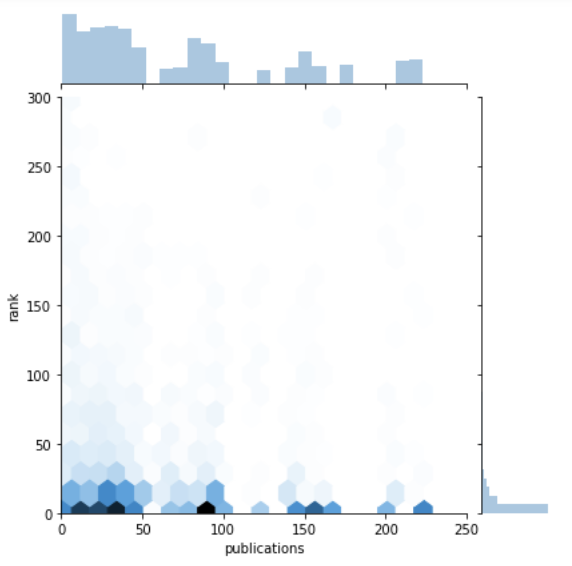
\includegraphics[width=.9\columnwidth]{./Train.png}

    Test
  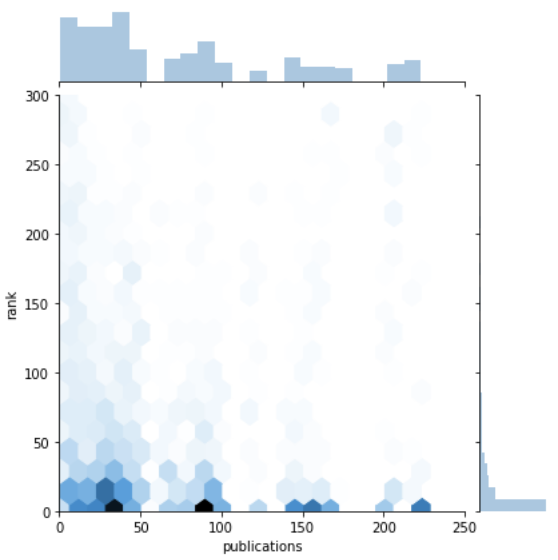
\includegraphics[width=.9\columnwidth]{./Test.png}
  \end{multicols}{2}
\end{frame}

\end{document}
